
\documentclass{amsart}

\usepackage{graphicx}
%\usepackage[altbullet]{lucidabr}
%two lines below change font (font intalled manually (i.e. uploaded))
%\usepackage{fontspec}
%\setmainfont[Ligatures=TeX]{LucidaBrightRegular.ttf}
%\usepackage{kpfonts}    % for nice fonts
% option [light] for more aery documents
\usepackage{color}  %for color of references
\usepackage[dvipsnames]{xcolor} %for color of references
\usepackage{caption}
\usepackage{fancyhdr}
\usepackage[pagebackref,colorlinks, citecolor=BlueViolet,urlcolor=BlueViolet]{hyperref}
\hypersetup{colorlinks = BlueViolet, allcolors = BlueViolet}
\usepackage[nameinlink,noabbrev]{cleveref} 
\usepackage{natbib}
\usepackage{multicol}
\usepackage{multirow}
%\usepackage{lscape}
\usepackage{pdflscape}
\usepackage{amssymb}
\usepackage{geometry}
\usepackage{longtable}
\usepackage{colortbl}
\usepackage{dsfont}
\usepackage{bm}
\usepackage{mathtools}
\usepackage{pgf}
\usepackage{tikz}
\usepackage{soul}
\usepackage{tikz}
\usepackage{tikz,fullpage}
\usepackage{pgf}
\usepackage{tikz}
\usepackage{bbm} %for the indicator function
\usetikzlibrary{shapes.geometric, arrows} %to create flow charts
\usepackage{bold-extra} %for bold small caps in the title
\usepackage{dirtree} % to create lists as tree

%\renewcommand{\familydefault}{\sfdefault} %for the sans serif font

%AMS original setup for mathematical elements
\newtheorem{theorem}{Theorem}[section]
\newtheorem{lemma}[theorem]{Lemma}
\theoremstyle{definition}
\newtheorem{definition}[theorem]{Definition}
\newtheorem{example}[theorem]{Example}
\newtheorem{xca}[theorem]{Exercise}
\theoremstyle{remark}
\newtheorem{remark}[theorem]{Remark}
\numberwithin{equation}{section}

%    Absolute value notation
\newcommand{\abs}[1]{\lvert#1\rvert}

%    Blank box placeholder for figures (to avoid requiring any
%    particular graphics capabilities for printing this document).
\newcommand{\blankbox}[2]{%
  \parbox{\columnwidth}{\centering
%    Set fboxsep to 0 so that the actual size of the box will match the
%    given measurements more closely.
    \setlength{\fboxsep}{0pt}%
    \fbox{\raisebox{0pt}[#2]{\hspace{#1}}}%
  }%
}

%Tikz setup for a flow chart
\tikzstyle{modelblock} = [rectangle, rounded corners, minimum width=3cm, minimum height=1cm,text centered, draw=black, fill=white, text ragged]

\tikzstyle{arrow} = [thick,->,>=stealth]

\begin{document}

\title{EC539 - Referee report}

%    Information for first author
\author{Arnaud Dy\`evre}
%\address{}
%\curraddr{}
%\email{a.dyevre@lse.ac.uk}
%\thanks{}

%    Information for second author
%\author{}
%\address{}
%\email{}
%\thanks{}

%    General info
%\subjclass[2000]{}

%\date{\today. First created October 19, 2019}

%\dedicatory{}
%\keywords{}

%\begin{abstract}

%\end{abstract}

\maketitle

\begin{center}
Student number: 201324680
\end{center}


\vspace{12pt}

Referee report of the journal article: \\ 
Kiyotaki, N., \& Moore, J. (2019). ``Liquidity, business cycles, and monetary policy''. \textit{Journal of Political Economy}, 127(6), 2926-2966.

%% The correct journal style for \specialsection is all uppercase; a known bug
%% in amsart.cls prevents this, so input must be uppercase until it is fixed.
%\specialsection*{This is a Special Section Head}
%\specialsection*{THIS IS A SPECIAL SECTION HEAD}
%This is an example of a special section head%
%%%%%%%%%%%%%%%%%%%%%%%%%%%%%%%%%%%%%%%%%%%%%%%%%%%%%%%%%%%%%%%%%%%%%%%%
%\footnote{Here is an example of a footnote. Notice that this footnote text is running on so that it can stand as an example of how a footnote with separate paragraphs should be written.
%\par
%And here is the beginning of the second paragraph.}%
%%%%%%%%%%%%%%%%%%%%%%%%%%%%%%%%%%%%%%%%%%%%%%%%%%%%%%%%%%%%%%%%%%%%%%%%
\newpage 

\subsection*{Summary of the paper} This article is an ambitious theoretical exploration of the role of liquidity in explaining asset prices and real quantity co-movements. Its main contribution is the introduction of a limit on the resale of equity in the budget constraint of investing entrepreneurs. In the most interesting case considered by the authors, which they call a ``monetary economy'', this buffer in the liquidation potential of entrepreneurs has \hl{X} important consequences (i) prevents the economy to reach its first best allocation of capital, (ii) leads entrepreneurs to hold precautionary money for no other reason than weathering times when they are illiquid, and (iii) monetary policy of the Quantitative Easing type reduces the impact of illiquidity on entrepreneurs' investment decisions. Two parameters and two types of assets lie at the centre of the model. With regards to parameters, $\theta$ is the share of furure earnings from the new capital an entrepreneur can credibly pledge, and $\phi$ is the share of equity they can convert into investable funds funds. Low $\omega$ and $\phi$ mean tight asset-based borrowing and liquidity constraints, respectively. The important assets are money, which is perfectly liquid but provide a low return, and equity, whose liquidity is determined by $\phi$ and which provide a return $r_t$. \\

The full model has two optimising agents, workers and entrepreneurs, and one rule-based agent, the government. The model is summarised graphically below.\\



More precisely, the central bank can exchange equity for money in period of illiquidity shock, and thus boost aggregate investment. 


Ultimately, the ambition of the paper is to create an ``LBC''--liquidity business cycl--model. 



\subsection*{Summary of the full model}. Given an aggregate state $\left(K_{t}, Z_{t}, N_{t}^{g}, a_{t}, \phi_{t}\right)$, and an exogenous law of motion for $\left(a_{t}, \phi_{t}\right)$, the model satisfies the following conditions:

\begin{tikzpicture}[node distance=cm, 
blocklarge/.style ={rectangle, rounded corners, draw=black, fill=white,  text centered, text width=27em},
blockmed/.style ={rectangle, rounded corners, draw=black, fill=white,  text centered, text width=20em},
block/.style ={rectangle, rounded corners, draw=black, fill=white,  text centered, text width=16em},
blockredlarge/.style ={rectangle, draw=red, fill=white,  text centered, text width=20em},
blockblue/.style ={rectangle, draw=blue, fill=white,  text centered, text width=16em}]
%, minimum height=4em

\node (workers) [blocklarge] {\textbf{Workers} (unit mass) \\
$$\max_{(C_t^w, L_t, N_{t+1}^w, M_{t+1}^w)} E_{t} \left[ \sum_{s=t}^{\infty} \beta^{s-t} U\left(C_{s}^{w}-\frac{\omega}{1+\nu}\left(L_{s}\right)^{1+\gamma}\right) \right]$$ \\
$$\mathrm{s.t.} \quad C_{t}^{w}+q_{t}\left(N_{t+1}^{w}-\lambda N_{t}^{w}\right)+p_{t}\left(M_{t+1}^{w}-M_{t}^{w}\right)=w_{t} L_{t}+r_{t} N_{t}^{u}$$
$$ N_{t+1}^{w} \geq\left(1-\phi_{t}\right) \lambda N_{t}^{w} \geq 0 $$
$$ M_{t+1}^{w} \geq 0 $$
};

\node (entrepreneurs) [block, below of=workers, yshift=-3.5cm] {\textbf{Entrepreneurs} (unit mass) \\
$$ \max_{\ell_t} A_{t} k_{t}^{\gamma} \ell_{t}^{1-\gamma}-w_{t} \ell_{t} -r_{t} k_{t}$$
};

\node (investing_entrepreneurs) [blocklarge, below of=entrepreneurs, yshift=-3.5cm] {\textbf{Investing Entrepreneurs} \\
Get investment opportunity with probability $\textcolor{red}{\pi}$
$$ \max_{c_t, \textcolor{red}{i_t}, k_{t+1}, n_{t+1}, m_{t+1}} E_{t} \sum_{s=t}^{\infty} \beta^{s-t} u\left(c_{s}\right)$$
$$\mathrm{s.t.} \quad c_{t}+\textcolor{red}{i_{t}}+q_{t}\left(n_{t+1}-\textcolor{red}{i_{t}}-\lambda n_{t}\right)+p_{t}\left(m_{t+1}-m_{t}\right)=r_{t} n_t$$
$$ n_{t+1} \geq \textcolor{red}{(1-\theta) i_{t}}+\left(1-\phi_{t}\right) \lambda n_{t}$$
$$m_{t+1} \geq 0$$
$$k_{t+1}=\lambda k_{t}+\textcolor{red}{i_{t}}$$ 
};

\node (storage) [block, right of=workers, xshift=9cm, yshift=-1cm] {\textbf{Storage} \\
$$\sigma\left(Z_{t+1}\right)=\left(\frac{Z_{t+1}}{\zeta_{0}}\right)^{\zeta}$$ 
};

\node (policy) [blockmed, right of=investing_entrepreneurs, xshift= 9cm, yshift=1cm] {\textbf{Monetary policy} \\
$$\frac{N_{t+1}^{g}}{K}=\psi_{a} \frac{a_{t}-a}{a}+\psi_{\phi} \frac{\phi_{t}-\phi}{\phi}$$
$$\mathrm{s.t.} \quad q_{t}\left(N_{t+1}^{g}-\lambda N_{t}^{g}\right) = r_{t} N_{t}^{g}+\left(\mu_{t}-1\right) B_{t}$$
$$K_{t+1}=N_{t+1}^{g}+N_{t+1}$$
};

%\node at (0,-7) (here) {test};

%\draw [arrow] (workers) -- node {$\quad \quad \ell_t^*$}(entrepreneurs)
%\draw [arrow] (entrepreneurs) -- node {$w_t^*$}(workers)
%\draw [arrow] (entrepreneurs) -- node {}(investing_entrepreneurs)

%\draw [->] (entrepreneurs) to[out=-80, in=-90,looseness=1] (here)    to[out=90,in=80,looseness=1] (workers);

\end{tikzpicture}



\subsection*{Position in the literature}. \cite{gertler2016wholesale}.

\subsubsection*{Intuition of the main result}

Monetary policy and storage are like pressure valves. Give intuition for equation (24).

\subsection*{Major comments} An interesting feature of the model is the interaction between asset prices and quantities. Standard RBC models and finance model do not have it.\\

\subsubsection{Putting the research in context} Until the Great Recession, most macroeconomic models treated financial constraints as being the problem of firms in the real economy only \citep{gertler2010financial}, and largely ignored the impact of liquidity constraints on economic activity. Furthermore, the Fed, the ECB, the Bank of England and many other large central banks engaged in unconventional policies that involved some form of direct lending in credit markets. The policy channel modelled by the authors is a direct theoretical counterpart to the Fed's expansion of the discount window loans, the Troubled Asset Relief Program, and the emergency loans to J.P. Morgan Chase (who absorbed Bear Stearns) and AIG.\\

Unlike standard RBC models, KM can generate substantial and long-lived responses in output, consumption, investment and capital utilisation without relying on implausibly large exogenous shocks. The amplification of the shock operates through the binding liquidity constraint \hl{More on this}.\\

Note that in the seminal \cite{kiyotaki1997credit} paper, the asset price moves little after a technology shock: it rises by 0.37\% following a 1\% increase in technology. In comparison, the price of money and the price of equity in \cite{kiyotaki2019liquidity} rise by 1.6 and 0.9\% respectively.\\

In general, DSGE models with credit constrained households manage to explain co-movements between house prices and consumption expenditures. But they have a hard time delivering co-movement between land prices and business investment \citep{iacoviello2010housing}. KM delivers this by assuming that entrepreneurs--rather than households/workers--are credit constrained, as \cite{liu2013land} do. The causal channel in both models is: a positive shock to land price raises firms' borrowing capacity, which in turns facilitates an expansion in investment and production. While this channel intuitively makes sense, the empirical study of \cite{lian2019anatomy} suggests that 83\% of large U.S. firms' corporate debt is based on cash flow from their operations (80\% in aggregate). It would thus have been helpful to show how important cash-flow-based debt is in Kiyotaki and Moore's model, compared to the liquidity and the investment-based (=future asset-based) borrowing constraints. One can think of a modified version of constraint (5) in their paper: $$n_{t+1} \geq(1-\theta) i_{t}+\left(1-\phi_{t}\right) \lambda n_{t} + (1-\delta)(y_t - w_t \ell_t) $$  \\
here $\delta$ would be the maximum share of equity on profit that an entrepreneur could issue.\\

Models such as \cite{bernanke1989agency} and \cite{kiyotaki1997credit} endogenise financial market frictions faced by actors in the real economy by creating an agency problem between lenders and borrowers. As a borrower's balance sheet deteriorate, their access to external finance becomes limited and they must bear most of the risk of the investment project with internal funds. The twoway interaction between investment and capital on the one hand, and access to credit on the other amplifies credit shocks. With the notable exception of \cite{holmstrom1997financial}, no macro-finance paper had thoroughly studied the theoretical implication of liquidity shortages in the financial sector. \\

\subsubsection*{Modelling the financial sector/endogenising the liquidity constraint} A notable omission of the paper is the absence of the financial sector as optimising agent. Modelling the mechanisms through which liquidity constraints emerge would have been an engaging addition to the paper. Understandably, the shocks that generate a tightening of the liquidity constraint could be many things (a sudden drop in trust in the inter-bank market, or the default of a large bank for instance), yet putting some behavioural structure on how the financial sector would react to these shocks could have painted a more comprehensive picture of liquidity-induced recessions. See \cite{he2013intermediary, angeloni2013capital, gertler2010financial} for recent work doing just this. I would have suggested to include a three-way interaction between workers (depositors), borrowers (firms) and the liquidity constraint (determined by the financial sector). In particular, it would have been nice to endogenise the agency problem created by the emergence of the central bank as a lender of last resort. Liquidity crises could be triggered by banks taking risky positions on the asset side of theuir balance sheet, under the assumption that they would be rescued by the government/the central bank.\\     

Using firm-level data, \cite{chaney2012collateral} find that for every dollar of increase in U.S. firms' real estate value, they are able to increase investment by 6 cents. This effect is even stronger for credit constrained firms. While this transmission channel has been highlighted by \cite{kiyotaki1997credit} already, its calibration to real data gives us a sense of its actual scale. \\

An important point for this type of research is to document which channel was the most important, liquidity constraints as suggested by this paper, or a more direct link between the housing market and business investment? Or maybe in which way did the interaction of the two lead to the crisis?\\

Another comment: scale of the liquidity shock. In their numerical exercise (part 3.), the authors use a drop in resaleability of the equity from 20\% to 6\%. More justifications about the specific magnitude of this drop would be helpful. Back-of-the-envelope calculations can help puting these results in perspective: a 20\% \\

Quantitatively, these unorthodox policies amounted to a lot: Federal Reserve (over US\$1.5 trillion, see Figure \ref{fig:fedsheet}) and the Bank of England (over £375 billion). It is worth noting, that when the thought of injecting liquid money into the economy buy buying off illiquid asset was first formulated by Kiyotaki and Moore as part of Moores's 2001 \textit{Clarendon Lectures}, the idea was deeply unconventional \citep{kiyotaki2001liquidity}. The Great Recession has been a spactacular confirmation of their vision.\\

Question the choice of preferences and technology. Are they linear? And if yes would the shock propagate similarly if these preferences were more traditional? \cite{cordoba2004credit} find that under concave preferences, concave technology and collateralised debt, collateral constraints can indeed amplify shocks, but these amplifications are relatively small. Large amplifications can be obtained under implausible parameter values, or worse, the equilibrium is not saddle path. More sensitivity analyses would have been welcomed to address such critiques.\\

The large interaction between the asset prices and quantity is an original feature of the model. This can be a powerful mechanism in the transmission of shocks to the broader economy.\\

The policy implications are evident with the hindsight of the Great Recession: the type of assets being traded on the inter-bank market matters, and their different liquidity (which are exacerbated by crises) can be trigger sever financial and real crises.

A lack of liquidity. The contagion of the recent financial crisis to the broader real economy. But are these liquidity constraints quantitatively big? \cite{liu2013land} have developed a DSGE model with land as a collateral asset and shocks driving most of the fluctuation in land prices. Their model is motivated by the fact that business investment dropped in tandem with land prices in the U.S. at the onset of the Great Recession.

\subsection*{Minor comments}

\subsection*{Suggested extension}

I believe the paper would have benefited from a model more directly applicable to monetary policy. Considering the importance of the liquidity channel in explaining important recent crises (Great Recession, the Greek debt crisis), \\

In this respect, a comparison of the model performance to the New Keynesian canon \citep{gali2015monetary} would have helped the reader in assessing the extent of the value added this model brings.\\

More fundamentally, my critique of the paper would be to treat the drop in liquidity as fully endogenous, and the liquidity constraint as fully reduced-form: dose-response? What make the liquidity of some asset change?\\

The model describe clearly the channel through which unorthodox monetary policy can dampen liquidity-induced recessions. Yet the effectiveness of this type of policy is mostly an empirical question. In this respect, I see this article as a first step in understanding the impact of liquidity constraints on asset prices and quantities. More needs to be done to quantify how important this cause of recession is. Its model desperately needs to be backed by some data. \hl{(suggest data extension)}. See \hl{cite} for some empirical explorations.\\

Even in the simplest version of the model, the liquidity constraint amplifies the impact of a productivity shock on aggregate consumption: without the binding liquidity constraint consumption would depend on permanent income rather than current income (see Figure 1 of the paper). But some authors have argued that liquidity constraints are not that powerful of a mechanism in amplifying productivity shocks \citep{cordoba2004credit}. It should be noted that th \\

The model's parsimony is one of its strengths, but I wonder how much interesting heterogeneity is hidden behind the representative agent assumption. A critique of the QE-type policies carried out by the ECB and the Fed after the 2008 crisis was that it surely helped financial institutions and kept the banking system afloat, but it increased the gap between the wealthiest and the poorest.\footnote{Adding heterogenity in previous-period wealth of labour income would however make the model much more complicated. I can understand why the authors kept it so streamlined.}
am also curious about the distributional aspects 

\subsubsection{Relationship to previous literature}

\subsection*{Relevance to policy debate}

\newpage

\bibliographystyle{ecta}
\bibliography{bibliography}

\newpage

\section*{Appendix}

\begin{figure}[h!]
    \centering
    \begin{tabular}{c}
        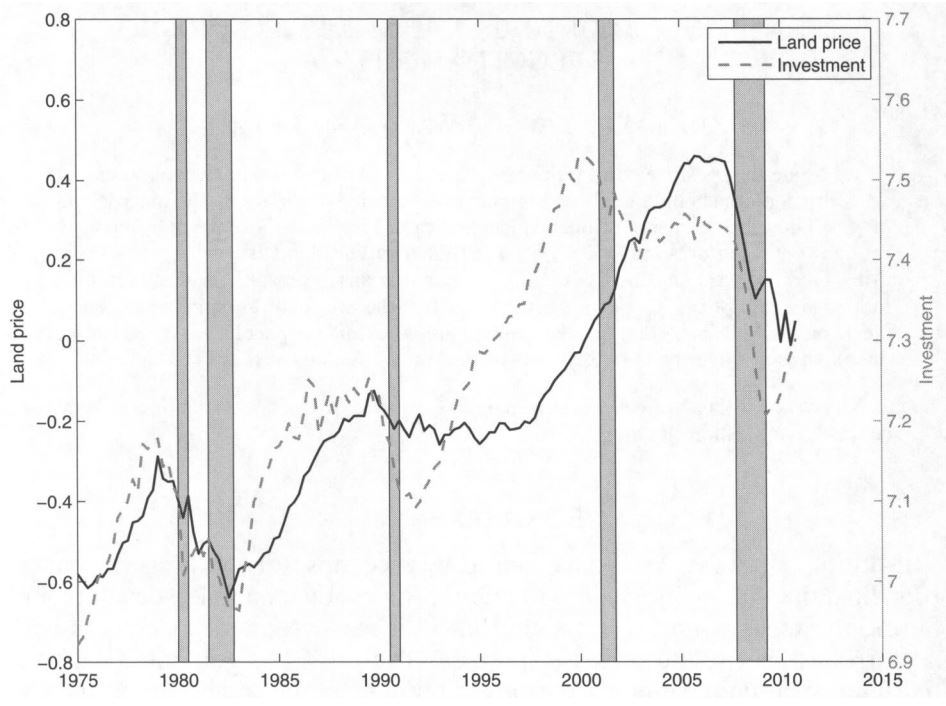
\includegraphics[width=0.8 \textwidth]{landpriceinvestment.JPG}
    \end{tabular}
    \caption{Real land price and investment (both in logs). Shaded areas are the NBER recession dates. Figure 1. from \cite{liu2013land}.}
    \label{fig:landpriceinvestment}
\end{figure}

\begin{figure}[h!]
    \centering
    \begin{tabular}{c}
        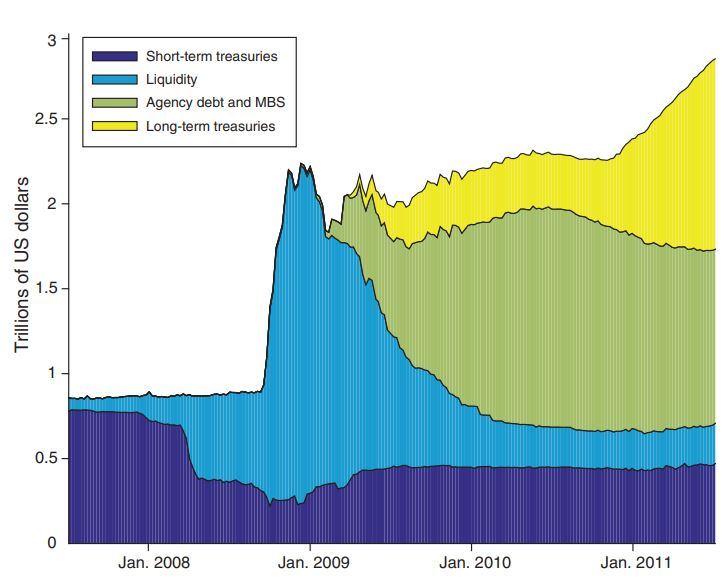
\includegraphics[width=0.8 \textwidth]{fedsheet.JPG}
    \end{tabular}
    \caption{federal Reserve's assets between July 2007 and July 2011.\\ Figure 1. from \cite{del2017great}}
    \label{fig:fedsheet}
\end{figure}

\end{document}

%------------------------------------------------------------------------------
% End of journal.tex
%------------------------------------------------------------------------------
